\documentclass[aspectratio=169,10pt,xcolor=table]{beamer}

\usepackage[utf8]{inputenc}
\usepackage[T1]{fontenc}
\usepackage[spanish]{babel}
\usepackage{booktabs}
\usepackage{graphicx}
\usepackage{tikz}
\usepackage{amsmath}
\usepackage{hyperref}
\usetikzlibrary{arrows.meta,positioning,shapes}

\usetheme{Madrid}
\definecolor{DARLblue}{RGB}{22,66,105}
\definecolor{DARLteal}{RGB}{28,132,137}
\definecolor{DARLgold}{RGB}{220,153,45}
\definecolor{DARLgray}{RGB}{80,88,96}
\definecolor{DARLred}{RGB}{176,58,46}
\setbeamercolor{structure}{fg=DARLblue}
\setbeamercolor{title}{fg=white,bg=DARLblue}
\setbeamercolor{frametitle}{fg=white,bg=DARLblue}
\setbeamercolor{block title}{fg=white,bg=DARLteal}
\setbeamercolor{block body}{fg=black,bg=black!4}
\setbeamercolor{block title alerted}{fg=white,bg=DARLred}
\setbeamercolor{block body alerted}{fg=black,bg=DARLred!6}
\setbeamertemplate{navigation symbols}{}
\setbeamertemplate{footline}[frame number]
\graphicspath{{../kaggle/dqn-dummy/v4/outputs/analisis/}{../thesis/images/}}

\newcommand{\hl}[1]{\textcolor{DARLblue}{\textbf{#1}}}

\title[DARL DQN Dummy v4]{DQN Dummy v4: cómo decide el agente\\y por qué desaprovecha A3}
\subtitle{Explicación del notebook, decisión trazada y oportunidades perdidas}
\author{Brigitte Dayane Rojas \and Jeffrey Antonio Monja}
\institute{Proyecto de tesis DARL}
\date{Corrida \texttt{jeffreyamc/darl-dqn-dummy-v4} · semilla 42 · checkpoint 940}

\begin{document}

\begin{frame}
  \titlepage
\end{frame}

% ---------------------------------------------------------------
\begin{frame}{Pregunta y mensaje principal}
\begin{block}{Pregunta de v4}
Cuando el cambio estadístico crece \textbf{gradualmente cada día}, ¿aprende el
agente \emph{cuándo} actuar y \emph{qué} etapa del pipeline actualizar?
\end{block}
\vspace{0.6em}
\begin{columns}[T]
\column{0.48\textwidth}
\textbf{Funciona}
\begin{itemize}
  \item Covariate: coincide con el oracle en \hl{15/15} decisiones.
  \item Con drift, recupera la AUC de 0,77--0,80 a \hl{0,90--0,93}.
  \item No actúa cuando no hay cambio.
\end{itemize}
\column{0.48\textwidth}
\textbf{Falla}
\begin{itemize}
  \item Aprovecha solo \textcolor{DARLred}{\textbf{1 de 10}} oportunidades de A3.
  \item Llega tarde al concept drift.
  \item Frente a la heurística: empata o pierde.
\end{itemize}
\end{columns}
\vspace{0.6em}
\begin{alertblock}{Hallazgo central}
Mientras la AUC está sobre 0,85, un día con concept drift produce
\textbf{la misma observación} que un día estable: el agente no puede distinguirlos.
\end{alertblock}
\end{frame}

% ---------------------------------------------------------------
\section{El notebook}
\begin{frame}{El notebook por bloques}
\centering
\begin{tikzpicture}[
  box/.style={draw=DARLblue, fill=DARLblue!8, rounded corners=2pt, align=center,
              minimum width=2.25cm, minimum height=1.05cm, font=\scriptsize},
  hid/.style={box, draw=DARLgold, fill=DARLgold!12},
  arr/.style={-{Stealth[length=2mm]}, thick, DARLgray}]
  \node[box] (data) {PhysioNet\\7 vitales};
  \node[box, right=0.45cm of data] (part) {Particiones\\A / B por paciente};
  \node[box, right=0.45cm of part] (lab) {Etiqueta\\\texttt{y\_dummy}};
  \node[box, right=0.45cm of lab] (rep) {Replay\\200 camas · 16 días};
  \node[hid, right=0.45cm of rep] (drift) {Drift gradual\\(oculto al agente)};
  \node[box, below=1.1cm of drift] (mon) {Monitor\\KS · PSI · AUC};
  \node[box, left=0.45cm of mon] (obs) {Estado\\30 valores};
  \node[box, left=0.45cm of obs, fill=DARLteal!15, draw=DARLteal] (dqn) {Double DQN\\elige A1--A4};
  \node[box, left=0.45cm of dqn] (pipe) {Pipeline\\mediana/IQR + XGBoost};
  \node[box, left=0.45cm of pipe] (rew) {Reward\\AUC$_{d+1}$ $-$ costo};
  \draw[arr] (data) -- (part); \draw[arr] (part) -- (lab); \draw[arr] (lab) -- (rep);
  \draw[arr] (rep) -- (drift); \draw[arr] (drift) -- (mon); \draw[arr] (mon) -- (obs);
  \draw[arr] (obs) -- (dqn); \draw[arr] (dqn) -- (pipe); \draw[arr] (pipe) -- (rew);
  \draw[arr, dashed] (rew.south) -- ++(0,-0.45) -| node[pos=0.25, below, font=\scriptsize] {aprende con la transición} (dqn.south);
\end{tikzpicture}
\vspace{0.8em}

\small Cada día: el monitor mide el pipeline actual $\rightarrow$ el agente elige
una acción al cierre $\rightarrow$ el día siguiente revela la recompensa.
\end{frame}

% ---------------------------------------------------------------
\begin{frame}{Datos, particiones y etiqueta artificial}
\begin{columns}[T]
\column{0.5\textwidth}
\textbf{Preparación de PhysioNet}
\begin{itemize}
  \item 40.336 pacientes y 1,55 M filas horarias.
  \item 7 vitales: HR, O2Sat, Temp, SBP, MAP, DBP y Resp.
  \item Faltantes: último valor del \emph{mismo} paciente (sin información futura).
\end{itemize}
\textbf{Particiones disjuntas por paciente}
\begin{itemize}
  \item Hospital A: 70/15/15 $\rightarrow$ modelo inicial.
  \item Hospital B: 60/20/20 $\rightarrow$ entrenar, validar y probar el agente.
  \item En B: pacientes de \emph{update} (para actualizar) y de \emph{eval} (para medir la AUC).
\end{itemize}
\column{0.5\textwidth}
\textbf{Etiqueta \texttt{y\_dummy}}
\begin{itemize}
  \item Score lineal de los 7 vitales normalizados.
  \item $y=1$ si el score supera la mediana; luego se invierte el 5\,\% al azar.
  \item Prevalencia 0,47. \textbf{No es la sepsis real}.
\end{itemize}
\textbf{Simulación temporal}
\begin{itemize}
  \item 100 camas de update y 100 de eval.
  \item Cuando un paciente termina, entra otro.
  \item 2.400 filas por día y rol, durante 16 días.
\end{itemize}
\end{columns}
\end{frame}

% ---------------------------------------------------------------
\begin{frame}{Pipeline, acciones y drift gradual}
\begin{columns}[T]
\column{0.47\textwidth}
\textbf{Pipeline de dos etapas}: normalización mediana/IQR recortada a $\pm 2$,
seguida de XGBoost (AUC 0,944 en A-test).
\vspace{0.4em}

\small
\begin{tabular}{@{}llr@{}}
\toprule
Acción & Qué hace & Costo \\
\midrule
A1 & No hacer nada & 0 \\
A2 & Recalcular mediana e IQR & 0,009 \\
A3 & Reentrenar XGBoost & 0,040 \\
A4 & A2 + A3 & 0,050 \\
\bottomrule
\end{tabular}

\vspace{0.3em}
\footnotesize Costo $= 0{,}05 \times$ segundos / segundos de A4.
\column{0.5\textwidth}
\textbf{Drift gradual (empieza el día 5)}
\begin{itemize}
  \item \textbf{Covariate}: desplaza los vitales 0,25 IQR por día.
  \item \textbf{Concept}: cambia 0,15 por día los pesos que definen la etiqueta.
  \item \textbf{Combined}: ambos; el concept empieza 2 días después.
\end{itemize}
\vspace{0.2em}
Las velocidades se calibran con B-train: caída $<0{,}05$ el primer día,
$>0{,}15$ tras 6 días y recuperación $>0{,}10$ al actuar.
\end{columns}
\end{frame}

% ---------------------------------------------------------------
\begin{frame}{Estado, recompensa y Double DQN}
\begin{columns}[T]
\column{0.5\textwidth}
\textbf{Estado: 30 valores}
\begin{itemize}
  \item Por día: KS máx., PSI máx. y AUC, cada uno en 3 categorías.
  \item Cortes de la AUC: $<0{,}65$ · $0{,}65$--$0{,}85$ · $\geq 0{,}85$.
  \item 10 valores por día $\times$ 3 días.
\end{itemize}
\textbf{Recompensa}
\[
r_d = \text{AUC}_{d+1} - \lambda\,\frac{t_a}{t_{A4}}
\]
\footnotesize Donde: $\text{AUC}_{d+1}$ es la AUC del día siguiente en
pacientes eval; $t_a$ son los segundos de la acción; $t_{A4}$ es la mediana de
A4; $\lambda=0{,}05$.
\column{0.47\textwidth}
\textbf{Double DQN (idea)}
\begin{itemize}
  \item La red estima un valor $Q$ por acción: la recompensa futura esperada.
  \item Se elige la acción con mayor $Q$.
  \item La red \emph{online} \textbf{elige} la acción siguiente y una copia
        congelada (\emph{target}) la \textbf{valora}. Eso reduce la sobreestimación.
\end{itemize}
\textbf{Entrenamiento}
\begin{itemize}
  \item Hasta 1000 episodios; 6 de cada 7 con drift.
  \item Día de inicio (3--7) y velocidad sorteados.
  \item Se elige el checkpoint 940 por validación.
\end{itemize}
\end{columns}
\end{frame}

% ---------------------------------------------------------------
\section{Resultados}
\begin{frame}{Resultado global en B-test}
\centering
\begin{tabular}{@{}lcccc@{}}
\toprule
Escenario & DQN & Heurística & No actuar (A1) & A3 fija \\
\midrule
Stable    & 14,106 & 14,106 & 14,106 & 13,342 \\
Covariate & \textbf{13,843} & 13,807 & 11,794 & 12,606 \\
Concept   & 13,382 & \textbf{13,405} & 11,369 & 13,271 \\
Combined  & \textbf{13,467} & 13,422 & 11,700 & 12,556 \\
\bottomrule
\end{tabular}

\vspace{0.3em}
\footnotesize Retorno = suma de 15 recompensas diarias (\texttt{policy\_comparison.csv}).
\normalsize
\vspace{0.8em}
\begin{columns}[T]
\column{0.47\textwidth}
\begin{block}{Lo positivo}
Supera claramente a no actuar y a cualquier acción fija en los tres escenarios con drift.
\end{block}
\column{0.47\textwidth}
\begin{alertblock}{Lo que no se puede afirmar}
Las diferencias con la heurística ($\leq 0{,}045$) son de una sola corrida; no
superan el ruido diario de la AUC.
\end{alertblock}
\end{columns}
\end{frame}

% ---------------------------------------------------------------
\section{Una decisión trazada}
\begin{frame}{Una decisión completa: concept, día 7}
\begin{columns}[T]
\column{0.48\textwidth}
\begin{block}{Lo que sabía el agente al decidir}
\begin{itemize}
  \item KS máx. 0,069 $\rightarrow$ \emph{bajo}.
  \item PSI máx. 0,020 $\rightarrow$ \emph{bajo}.
  \item AUC del día 0,862 $\rightarrow$ \emph{alta} ($\geq 0{,}85$).
  \item Días 5 y 6 iguales: AUC 0,944 y 0,907.
\end{itemize}
$Q$: A1 \textbf{1,502} · A2 1,458 · A3 1,422 · A4 1,455\\
$\Rightarrow$ elige \textbf{A1}.
\end{block}
\column{0.48\textwidth}
\begin{alertblock}{Lo que se conoce después (auditoría)}
\begin{itemize}
  \item Severidad oculta del concept: 0,45.
  \item AUC del día 8 con A1: \textbf{0,810}; costo $\approx 0$; reward 0,810.
  \item Oracle (las 4 acciones sobre el mismo día 8):\\
        A1 0,810 · A2 0,786 · \textbf{A3 0,876} · A4 0,863.
  \item \emph{Regret} $= 0{,}066$, el mayor del experimento.
\end{itemize}
\end{alertblock}
\end{columns}
\vspace{0.6em}
\centering
\small Los valores $Q$ son \textbf{exactamente iguales} a los de un día del escenario stable.
\end{frame}

% ---------------------------------------------------------------
\begin{frame}{Concept: el agente espera hasta que la AUC cruza 0,85}
\centering
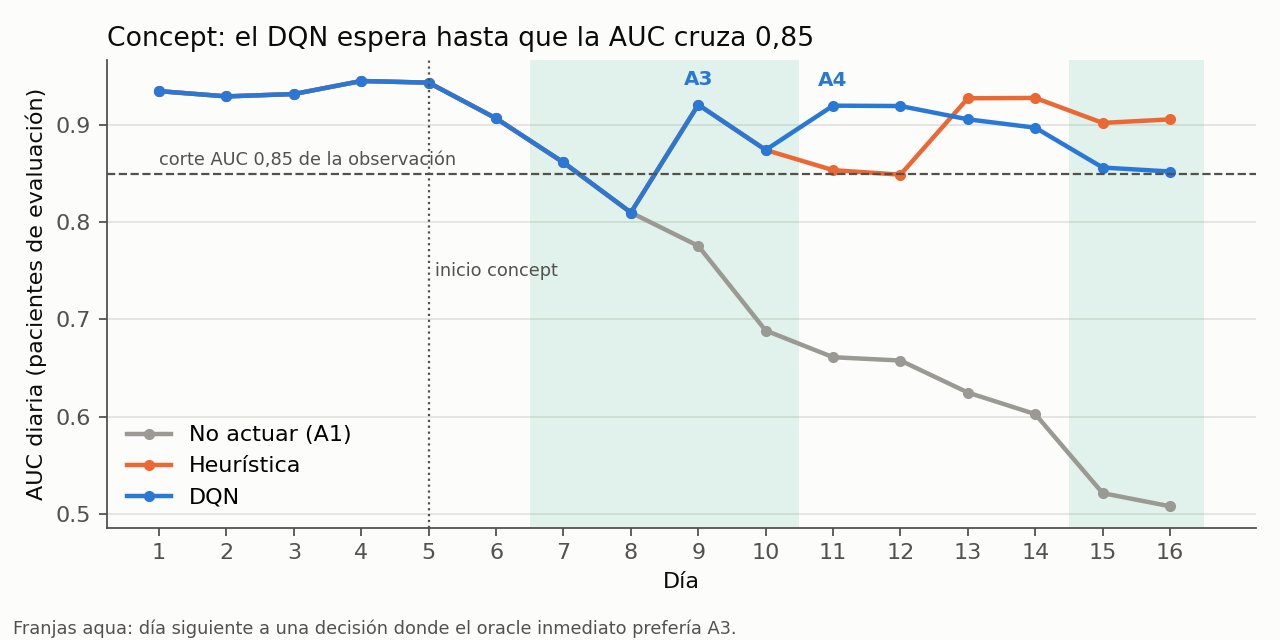
\includegraphics[width=0.78\textwidth]{A_concept_auc_dqn_heuristica.png}

\small
Sin actuar, la AUC cae de 0,94 a 0,51. El DQN y la heurística siguen la misma
curva hasta el día 8: ninguno actúa mientras la AUC está sobre el corte.
En los días 14--15 vuelve a caer y el DQN no reacciona.
\end{frame}

% ---------------------------------------------------------------
\begin{frame}{No es que decida esperar: no puede ver la diferencia}
\centering
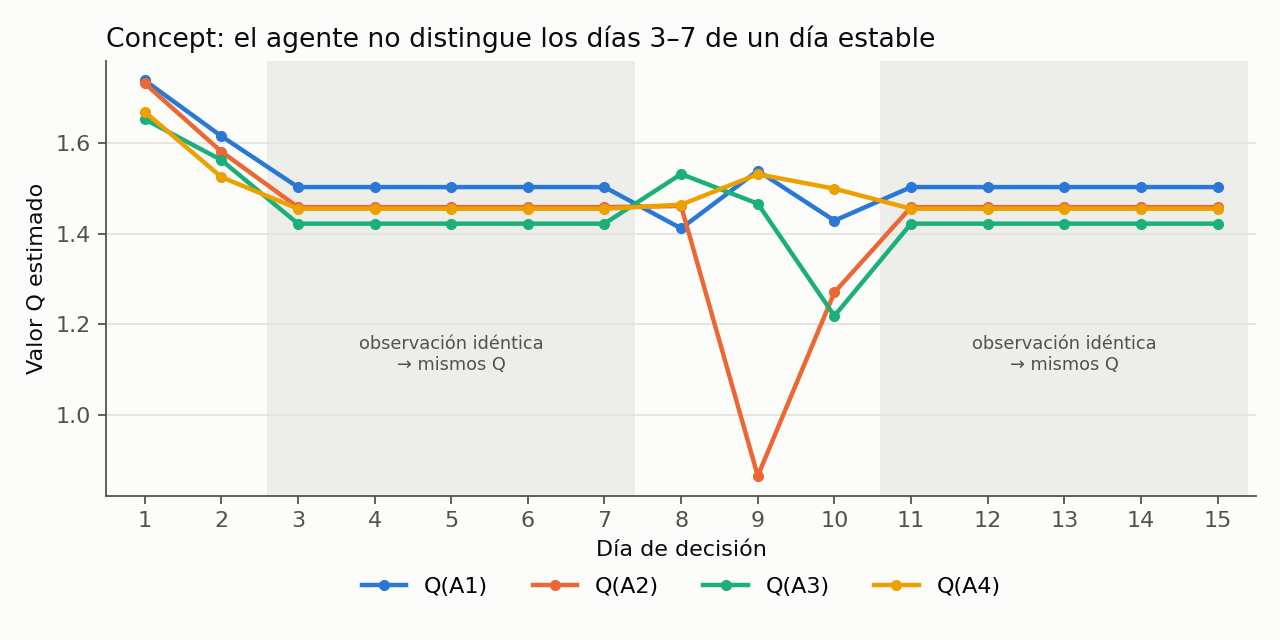
\includegraphics[width=0.74\textwidth]{B_concept_valores_q.png}

\small
En los días 3--7 y 11--15 los valores $Q$ quedan planos: la entrada es la misma
que en un día estable. $Q(\text{A3})$ solo supera a $Q(\text{A1})$ el día 8,
cuando la AUC pasa a la categoría media.
\end{frame}

% ---------------------------------------------------------------
\section{Oportunidades A3}
\begin{frame}{Tabla de oportunidades: días donde el oracle prefería A3}
\centering
\footnotesize
\begin{tabular}{@{}llcccccc@{}}
\toprule
Escenario & Día & Elegida & Util. A3 & Util. elegida & Regret & AUC obs. & KS / PSI \\
\midrule
Concept  & 6  & A1 & 0,878 & 0,862 & 0,017 & 0,907 & 0,07 / 0,02 \\
\rowcolor{DARLgold!20}
Concept  & 7  & A1 & 0,876 & 0,810 & \textbf{0,066} & 0,862 & 0,07 / 0,02 \\
Concept  & 8  & A3 & 0,879 & 0,879 & 0,000 & 0,810 & 0,06 / 0,03 \\
Concept  & 9  & A1 & 0,885 & 0,874 & 0,011 & 0,921 & 0,07 / 0,02 \\
Concept  & 14 & A1 & 0,882 & 0,856 & 0,026 & 0,897 & 0,08 / 0,05 \\
Concept  & 15 & A1 & 0,894 & 0,852 & 0,042 & 0,856 & 0,09 / 0,05 \\
\rowcolor{DARLgold!20}
Combined & 9  & A2 & 0,883 & 0,837 & \textbf{0,046} & 0,887 & 0,23 / 0,14 \\
Combined & 10 & A4 & 0,878 & 0,870 & 0,008 & 0,846 & 0,23 / 0,22 \\
Combined & 12 & A2 & 0,880 & 0,838 & 0,043 & 0,890 & 0,35 / 8,19 \\
\rowcolor{DARLgold!20}
Combined & 13 & A4 & 0,886 & 0,877 & \textbf{0,009} & 0,847 & 0,26 / 0,15 \\
\bottomrule
\end{tabular}

\vspace{0.6em}
\small Aprovecha 1 de 10 oportunidades. \emph{Regret} total en las 9 restantes: \textbf{0,27}.
\end{frame}

% ---------------------------------------------------------------
\begin{frame}{Tres casos, tres tipos de fallo}
\begin{columns}[T]
\column{0.32\textwidth}
\begin{block}{Concept, día 7}
\textbf{No ve el problema.}\\[0.3em]
La AUC (0,862) sigue sobre 0,85, así que el estado es igual a un día estable.
Ahí A3 casi siempre pierde: cuesta 0,04 y, sin drift, reentrenar con un día baja
la AUC (0,940 $\rightarrow$ 0,932).\\[0.3em]
\emph{Regret} 0,066.
\end{block}
\column{0.32\textwidth}
\begin{block}{Combined, día 9}
\textbf{Confunde el tipo de cambio.}\\[0.3em]
KS 0,23 y PSI 0,14 parecen covariate, y la AUC (0,887) aún es alta. Elige A2
($Q$ 1,136 frente a 1,015 de A3), pero el concept ya va en 0,45 y solo A3 lo
corrige.\\[0.3em]
\emph{Regret} 0,046.
\end{block}
\column{0.32\textwidth}
\begin{block}{Combined, día 13}
\textbf{Acierta, pero paga de más.}\\[0.3em]
La AUC (0,847) bajó del corte y elige A4 ($Q$ 0,956). A4 incluye A3 y logra la
misma AUC ($\approx 0{,}929$); la pérdida es solo la diferencia de costo entre A4
y A3.\\[0.3em]
\emph{Regret} 0,009.
\end{block}
\end{columns}
\end{frame}

% ---------------------------------------------------------------
\begin{frame}{Cuánto se perdió en cada oportunidad}
\centering
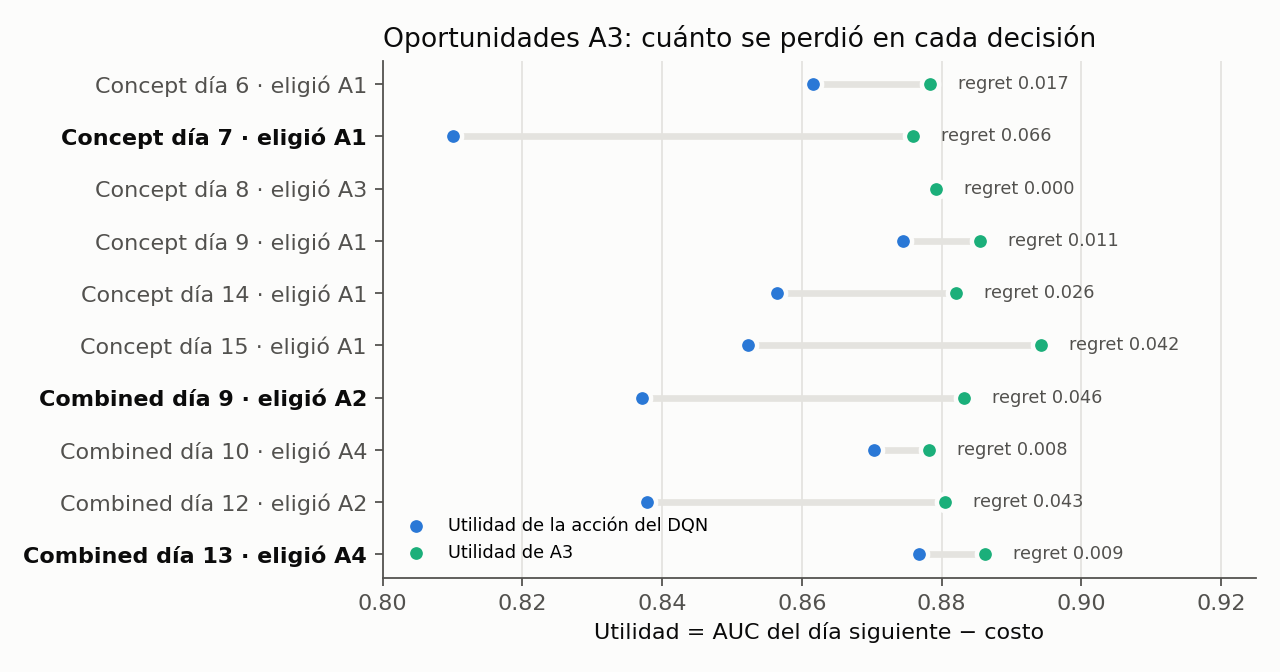
\includegraphics[width=0.8\textwidth]{C_oportunidades_a3_regret.png}

\small
Las pérdidas grandes ($\geq 0{,}04$) ocurren cuando la AUC aún está sobre 0,85
(concept 7 y 15) o cuando las señales de covariate tapan el concept (combined 9 y 12).
\end{frame}

% ---------------------------------------------------------------
\begin{frame}{Lo que muestra el entrenamiento}
\begin{columns}[T]
\column{0.48\textwidth}
\textbf{A3 se usa cada vez menos}
\begin{itemize}
  \item Elección de A3 en entrenamiento: \hl{21\,\%} $\rightarrow$ \hl{7\,\%}.
  \item En validación: de $\sim$14 a $\sim$3--5 decisiones de 60.
  \item En los estados donde se prueba, A3 casi siempre pierde, así que el
        agente deja de elegirla.
\end{itemize}
\column{0.48\textwidth}
\textbf{La política no se estabiliza}
\begin{itemize}
  \item Coincidencia entre checkpoints consecutivos: 0,37--0,74 por bloque de
        100 episodios.
  \item Baja hasta \textcolor{DARLred}{\textbf{0,35}} cerca del final.
  \item Gate \texttt{validation\_converged}: \textcolor{DARLred}{\textbf{no cumplido}} (85\,\% frente a 95\,\%).
\end{itemize}
\end{columns}
\vspace{0.8em}
\begin{block}{Además}
El costo medido de A3 varía entre 0,036 y 0,081 según la CPU de Kaggle: el
reward incluye ruido del hardware.
\end{block}
\end{frame}

% ---------------------------------------------------------------
\section{Conclusiones}
\begin{frame}{Posibles explicaciones}
\begin{enumerate}
  \item \textbf{Estados indistinguibles} (la más respaldada).
        El corte de AUC en 0,85 junta los días con concept temprano y los días
        estables. Comprobado: los valores $Q$ son idénticos.
  \item \textbf{Señales mezcladas en combined.}
        KS y PSI solo miden el cambio de medición; cuando aparecen, el agente
        atribuye la caída a covariate.
  \item \textbf{A3 se refuerza poco.}
        Se prueba sobre todo en estados donde pierde, y su uso cae del 21\,\% al 7\,\%.
  \item \textbf{Ruido en el reward.}
        La variación del costo de A3 es mayor que muchas de las diferencias que
        el agente debe aprender.
\end{enumerate}
\end{frame}

% ---------------------------------------------------------------
\section{Experimento rápido}
\begin{frame}{Experimento sin entrenar: ¿actuar antes con A3 mejora el episodio?}
\small
Mismo código del v4, \textbf{20 replays} de B-test, costo fijo por acción y
\textbf{ningún DQN entrenado}. Se cambia solo la regla de decisión.
\vspace{0.4em}

\centering
\footnotesize
\begin{tabular}{@{}lcccc@{}}
\toprule
Diferencia vs. heurística v4 & Corte 0,90 & Caída AUC $\geq 0{,}03$ & Oracle miope$^{*}$ & Periódica (A3 c/3 días) \\
\midrule
Stable    & 0,000 & 0,000 & 0,000 & $-0{,}314$ \\
Covariate & $-0{,}009 \pm 0{,}012$ & $-0{,}029 \pm 0{,}019$ & $+0{,}023$ & $-0{,}103$ \\
\rowcolor{DARLgold!20}
Concept   & $\mathbf{+0{,}137 \pm 0{,}021}$ & $\mathbf{+0{,}116 \pm 0{,}022}$ & $+0{,}166$ & $+0{,}036$ \\
\rowcolor{DARLgold!20}
Combined  & $\mathbf{+0{,}140 \pm 0{,}037}$ & $\mathbf{+0{,}114 \pm 0{,}047}$ & $+0{,}202$ & $-1{,}105$ \\
\bottomrule
\end{tabular}

\vspace{0.2em}
\raggedright
\scriptsize $^{*}$ Usa etiquetas futuras: es solo una referencia. Valores: media de diferencias pareadas $\pm$ IC 95\,\%.
\normalsize
\vspace{0.6em}
\begin{columns}[T]
\column{0.48\textwidth}
\begin{block}{Lectura}
Con corte 0,90 la primera A3 llega el día 7 (antes, el 8) y gana en
\textbf{20/20} replays de concept. Captura el 83\,\% de la ventaja del oracle.
Sin drift no genera falsas alarmas.
\end{block}
\column{0.48\textwidth}
\begin{alertblock}{Límite}
Los cortes 0,90 y 0,03 se eligieron a mano y se midieron en B-test.
Para la tesis hay que elegirlos en B-val.
\end{alertblock}
\end{columns}
\end{frame}

% ---------------------------------------------------------------
\begin{frame}{Una corrida no basta; la información sí está en la AUC}
\centering
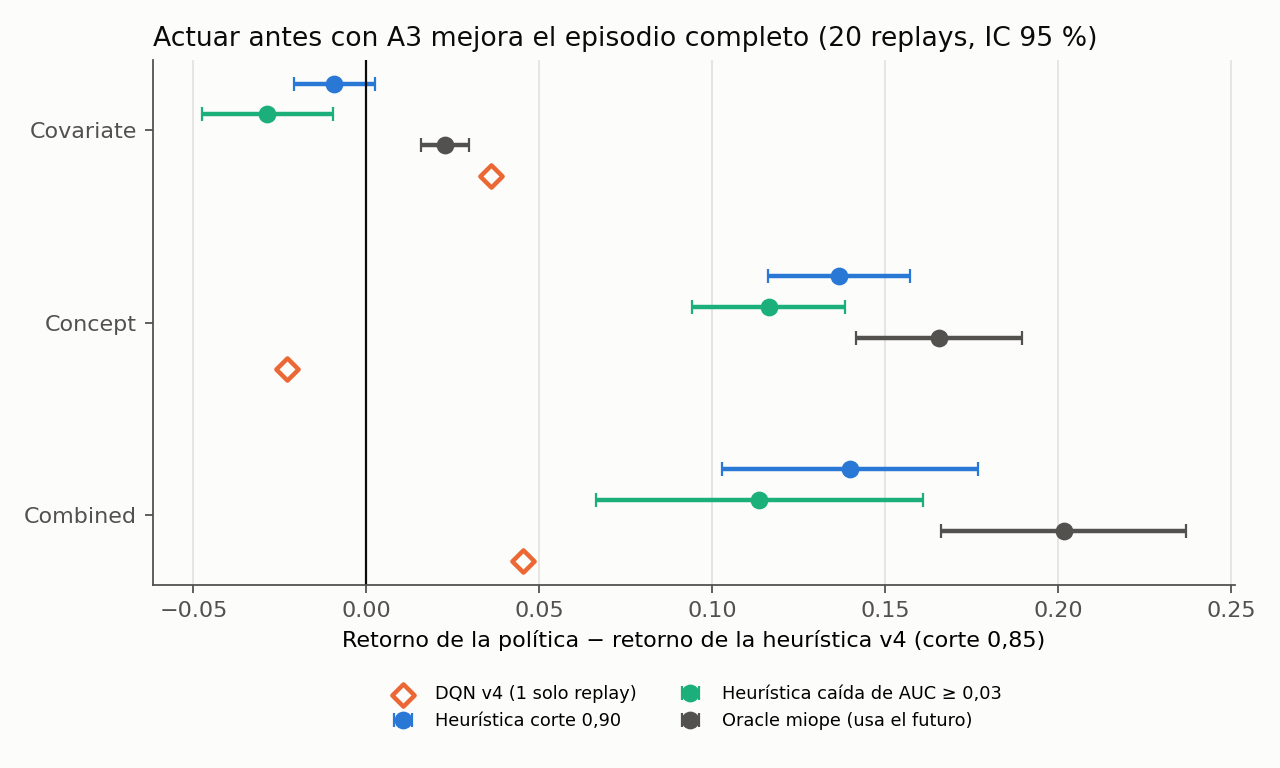
\includegraphics[width=0.6\textwidth]{exp_heuristicas/D_diferencia_vs_heuristica.png}

\small
\begin{itemize}
  \item En el \textbf{mismo replay} del v4, la heurística 0,90 supera al DQN en concept
        (13,555 vs. 13,382) y en combined (13,555 vs. 13,467).
  \item Entre replays, la diferencia pareada varía 0,04--0,10: las diferencias
        DQN--heurística del v4 ($\leq 0{,}045$) no son concluyentes.
\end{itemize}
\end{frame}

% ---------------------------------------------------------------
\begin{frame}{Evidencia que falta y próximos pasos}
\begin{columns}[T]
\column{0.48\textwidth}
\begin{alertblock}{Evidencia que falta}
\begin{itemize}
  \item \textbf{Ya respondido}: actuar antes con A3 sí mejora el episodio
        completo (experimento sin entrenar).
  \item \textbf{Elegir los cortes en B-val} y confirmar en B-test.
  \item \textbf{Confirmar la explicación 1 con el DQN}: reentrenarlo con
        observación continua y evaluarlo en los 20 replays.
\end{itemize}
\end{alertblock}
\column{0.48\textwidth}
\begin{block}{Propuesta para v5}
\begin{itemize}
  \item Observación con métricas \textbf{continuas}, última acción y días desde
        la última actualización.
  \item \textbf{Costo fijo} por acción en lugar del tiempo medido.
  \item Evaluación con varias semillas, IC 95\,\% y baseline periódico.
  \item Etiqueta con 1 día de retraso, como en la tesis.
\end{itemize}
\end{block}
\end{columns}
\vspace{0.6em}
\centering
\small Los signos vitales son reales; la etiqueta y el drift son sintéticos.
No es una validación clínica.
\end{frame}

\end{document}
